Text embedding models anchor retrieval, retrieval-augmented generation (RAG)~\cite{rag}, and classification pipelines whose vector indexes depend on a stable embedding geometry.
At the same time, search workloads increasingly require images, including screenshots, page scans, infographics, and other rendered media; audio, such as speech, music, and natural sounds; as well as video, to be queried alongside text.~\cite{mieb,vidore,mmeb,maeb}
%This creates a tension: multimodal embedders should broaden the modality coverage of retrieval systems, but changing the text embedding space invalidates existing text indexes and makes comparisons to the source text-only embedding model ambiguous.

\begin{figure}[t]
  \centering
  \vspace{0.75\baselineskip}
  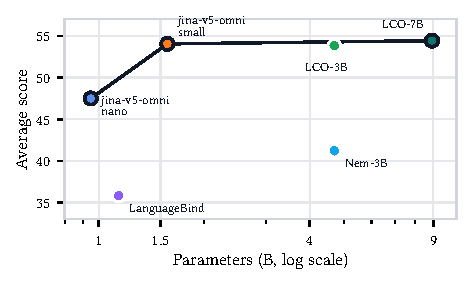
\includegraphics[width=\columnwidth]{figures/omni_average_frontier.pdf}
  \caption{Average performance across multimodal embedding tasks versus model parameter count (see Table~\ref{tab:omni-frontier}).}
  \Description{A one-column frontier chart with Table 1 average scores for six open-weight omni models: jina-v5-omni-nano, jina-v5-omni-small, LanguageBind, LCO-3B, LCO-7B, and Nem-3B.}
  \label{fig:omni-average-frontier}
\end{figure}

\begin{figure*}[!t]
\centering

\includegraphics[width=\textwidth]{figures/openai_image_2/architecture.png}
\caption{Architecture of \omniBase{} (\omniSmall{} shown; \omniNano{} uses a smaller ViT and LLaVA-style tokens).
Frozen towers feed trainable modality projectors into the frozen text backbone; task-specific exports select one projector/delimiter set and the matching LoRA adapter.}
\label{fig:architecture}
\end{figure*}

We present \omniBase{}, a pair of models that extends a text embedding backbone to image, video, and audio while leaving the model entirely unchanged for text inputs. The two models differ substantially in size: \omniNano{} is based on \textNano{}, with 0.24B parameters in its base text-only model, and \omniSmall{}, based on \textSmall{} with 0.67B parameters.~\cite{jina-v5-text} 
The two base models have already been trained for high-performance text embeddings, using LoRA adapters to optimize them for multiple tasks: retrieval, text-matching, clustering, and classification. 

To add support for non-text modalities, we integrate:
\begin{itemize}
    \item Vision encoders from Qwen3.5-2B and Qwen3.5-0.8B~\cite{qwen3.5}, which have been adapted from SigLIP2 So400m and SigLIP2 Base respectively.~\cite{siglip2}
    \item The Qwen2.5-Omni audio encoder,~\cite{qwen2.5-omni} which has been adapted from Whisper-large-v3.~\cite{whisper}
\end{itemize}

The core idea of GELATO is to use independently pretrained, language-aligned encoders and align them to text embedding models through small trainable projectors rather than jointly retraining them. This makes it possible to readily construct modular multimodal embedding models while minimizing added parameters and additional training.

\paragraph{Contributions.}
\begin{enumerate}
  \item We describe GELATO and apply it in the construction of the \omniBase{} model suite by extending the Jina Embeddings v5 Text suite to support other media.
  \item We contribute to the open embedding ecosystem by releasing the \omniBase{} model collection\footnote{\href{https://huggingface.co/collections/jinaai/jina-embeddings-v5-omni-69f336b985c156b1d757029e}{Jina Embeddings v5 Omni Hugging Face collection}.}, comprising two base models and eight task-specific variants for retrieval, classification, clustering, and text-matching across Small and Nano scales.
  \item We evaluate \omniBase{} and comparable models across a range of standard benchmarks, and show that GELATO produces competitive results. (See Figure~\ref{fig:omni-average-frontier}.)
  \item We analyze the design rules behind GELATO through ablations on projector training, encoder choice, and Matryoshka truncation, and separately quantify training efficiency.
\end{enumerate}
